% !TEX root = ../thesis.tex
% testing and optimization experiments
% @author Tobias Wulf
%

\chapter{Erprobungs- und Optimierungsexperimente 0.0.1 13.01.2021}\label{ch:erprobungs-u-opt-exp}
	\begin{itemize}
		\item Klassifizierung (Diagnose)
		\item Stabilitätskriterium
		\item Fehlererkennung Max. Mittelwert, Qualitätsmaß
		\item Allg. Vorgehen "Batch-Job"
		\item Konfigurierung der Simulationssoftware
	\end{itemize}

\section{Festlegung des Startpunktes}\label{sec:festlegung-des-startpunktes}
	\begin{itemize}
		\item Startpunkt, 1. Position gleich Anlernpunkt für Trainingsphase
		\item Auswahl des Senortyps
		\item Konfigurierung des Magneten
		\item Auswahl des GPR-Modells nach Optimierung
		\item Konfigurierung des GPR-Modells mit ermittelten Parametern
	\end{itemize}



\begin{figure}[tbph]
	\centering
	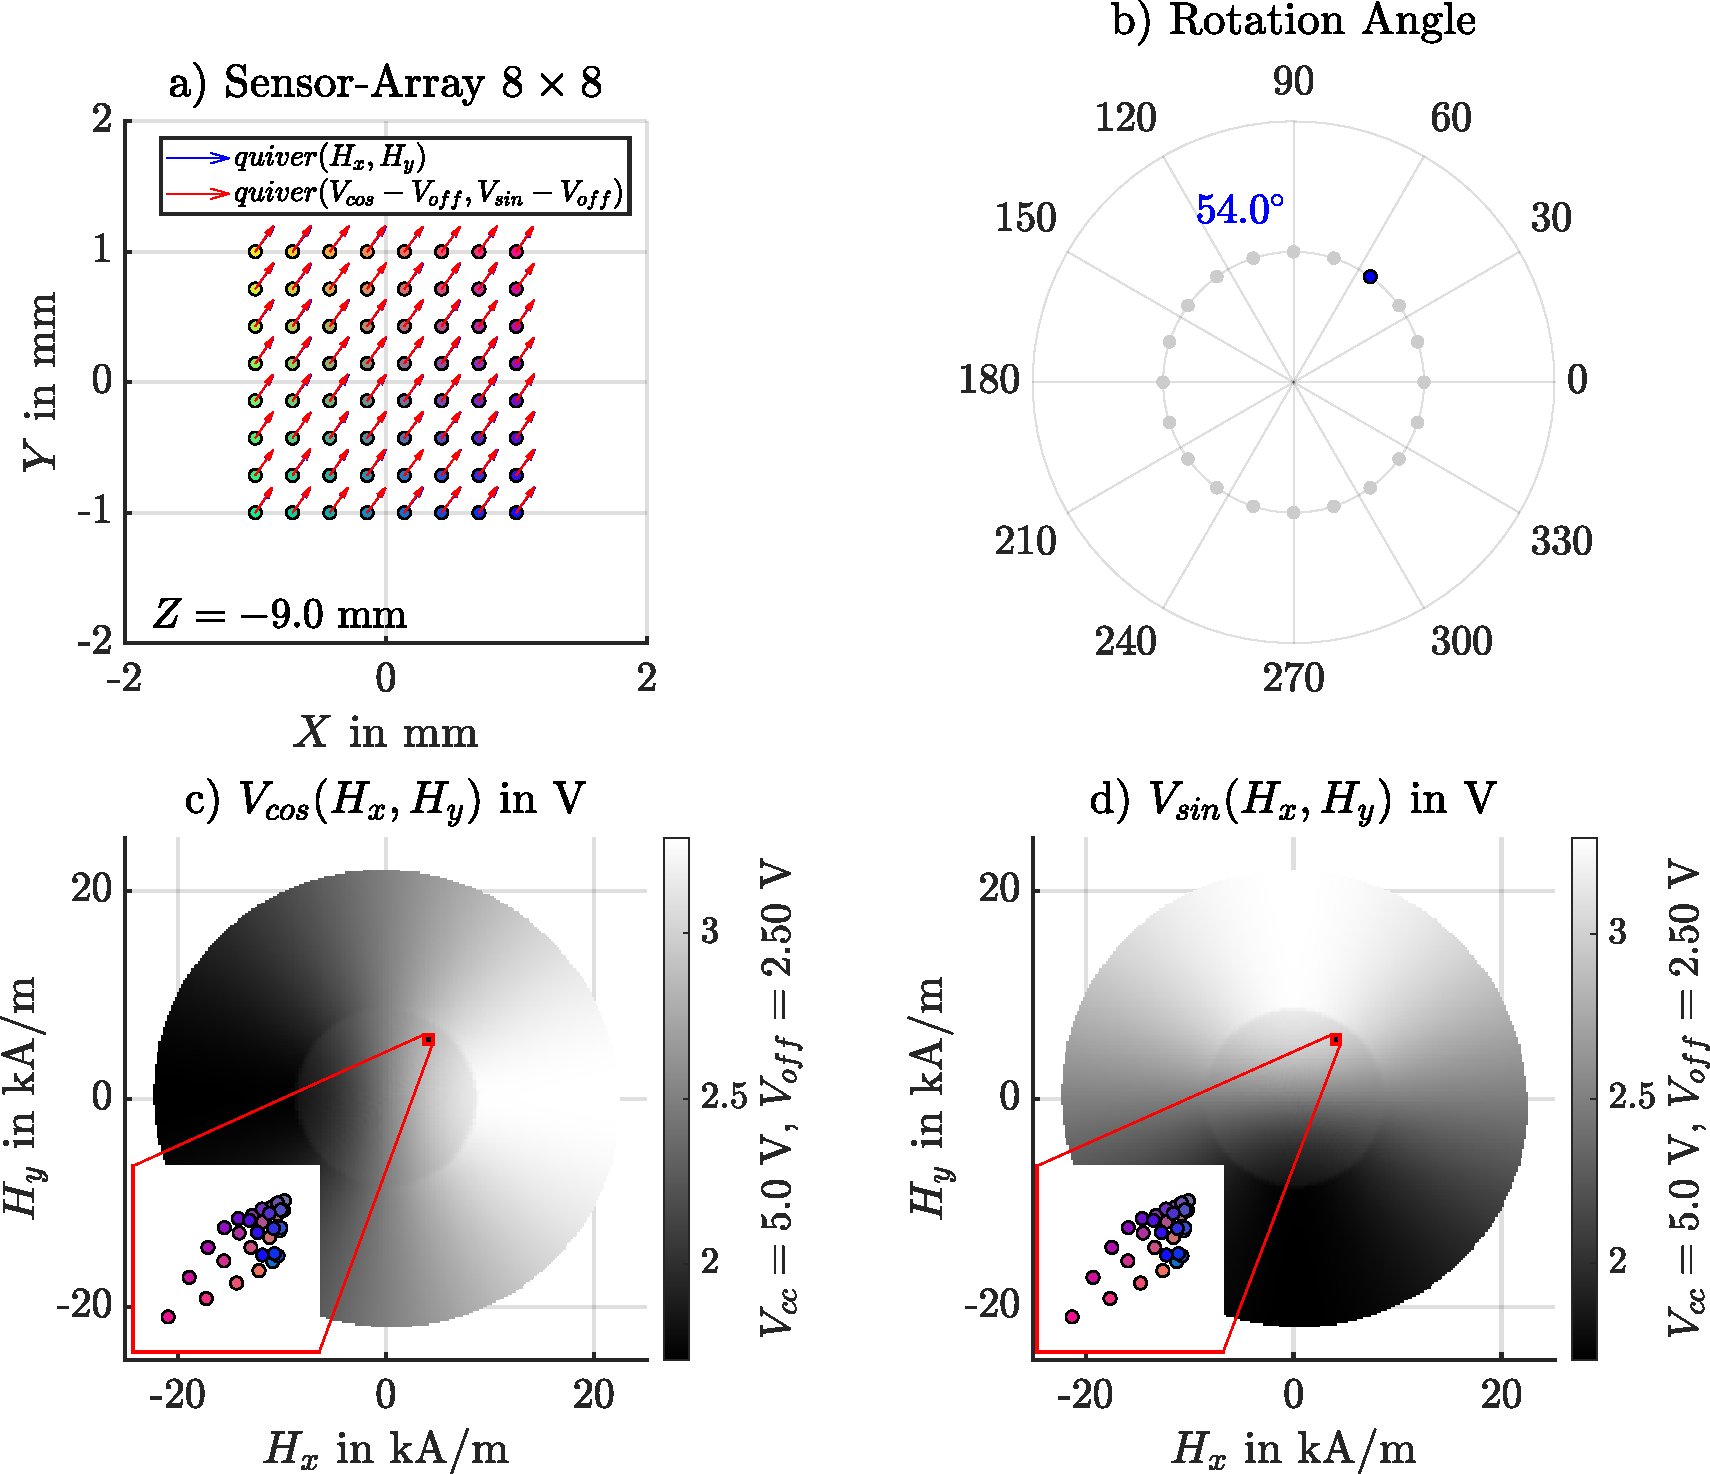
\includegraphics[width=.95\linewidth]{chapters/images/4-EuOExp/Kennfeld-Mapping}
	\caption[Kennfeld-Mapping]{Kennfeld-Mapping}
	\label{fig:kennfeld-mapping}
\end{figure}

\begin{figure}[tbph]
	\centering
	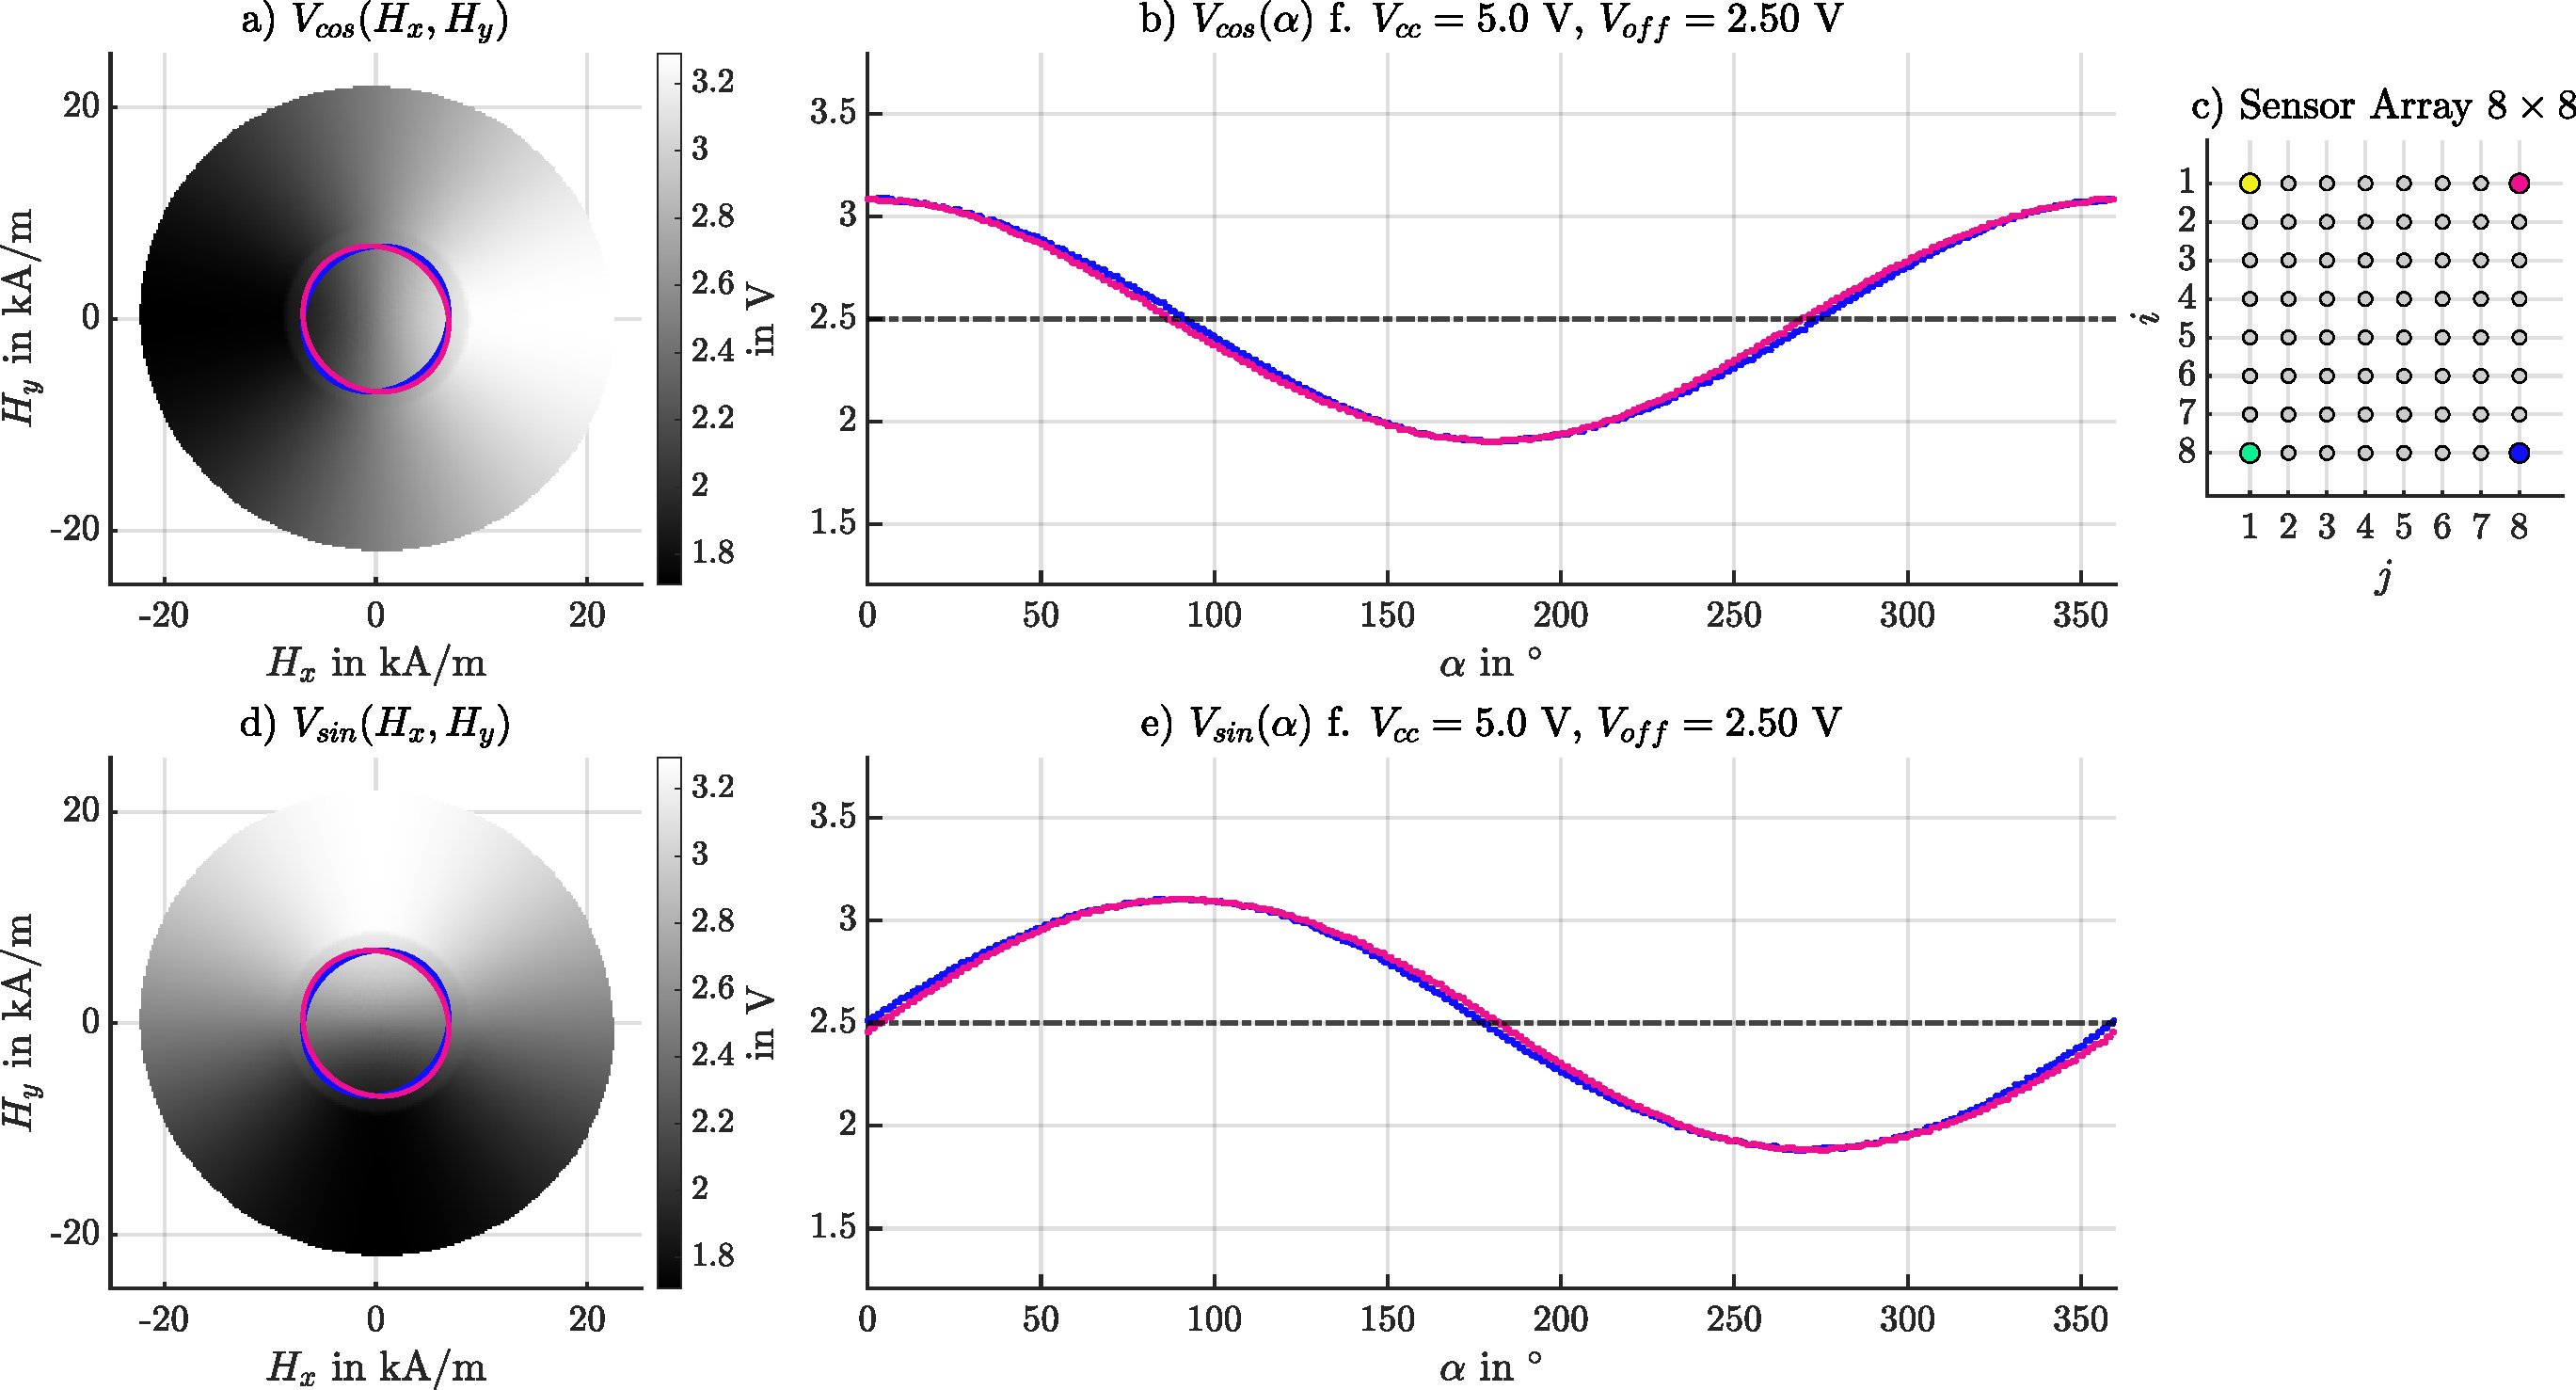
\includegraphics[width=\linewidth]{chapters/images/4-EuOExp/Senor-Array-Teilansicht}
	\caption[Sensor-Array Teilansicht]{Sensor-Array Teilansicht}
	\label{fig:senor-array-teilansicht}
\end{figure}

\section{Festlegung des Verfahrweges ohne Verkippung}\label{sec:festlegung-verfahrwe-ohne-verkippung}
	\begin{itemize}
		\item Vorbetrachtung des Magnetsfeldes 
		\item Aufteilung in Sektoren
		\item Abfahren in Z-Richtung ohne Versatz
		\item Festlegen des X-Y-Versatzes, Symmetrie-Sektor		
	\end{itemize}

\section{Simulationsdurchführung}\label{sec:simulationsdurchfuehrung}
	\begin{itemize}
		\item Festhalten der Ergebnisse
		\item Position, Winkelfehler (Max, Mittel), Qualitätsmaß (Max, Mittel)
		\item Drift-Darstellung
	\end{itemize}
	
